
\section{3D coordinate phase-cycle \texorpdfstring{$\delta_3$}{delta3} fixture specification}\label{manual:app:coordinate-phase-cycle-delta3}
This appendix records the active integer 3D coordinate fixture used by time-ordered trajectory records. It gives the coordinate-level specification: integerized trajectory bins, squared displacement counts, phase-cycle counts, octant counts, integer ratios, and exact \(\delta_3\) residuals. Continuous-motion summaries are downstream presentation maps and do not enter the exact fixture.

\begin{figure}[H]
\centering
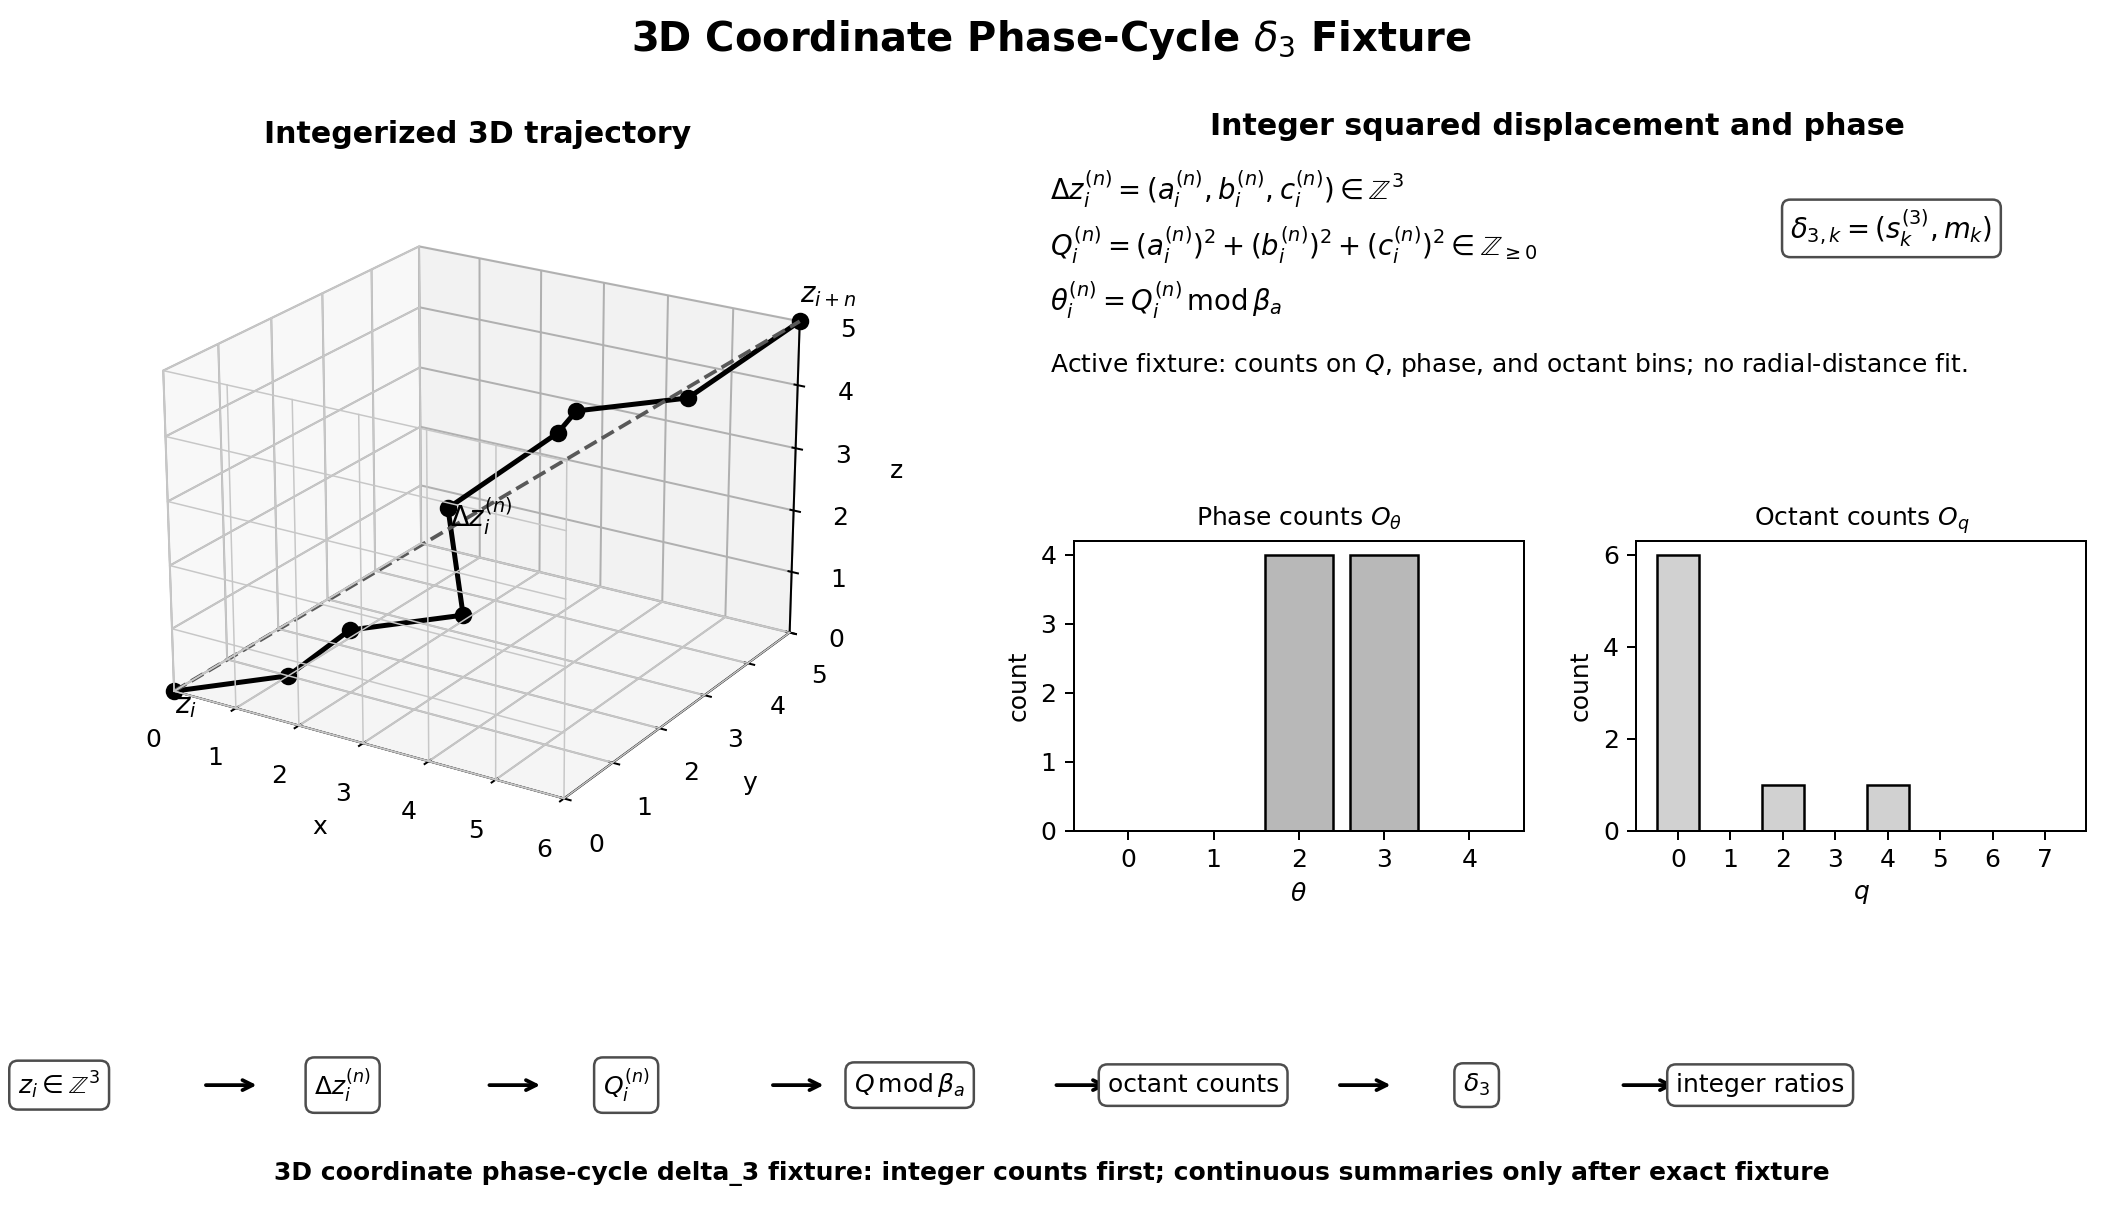
\includegraphics[width=0.95\linewidth]{figures/coordinate_phase_delta3_wireframe.png}
\caption{3D coordinate phase-cycle \(\delta_3\) fixture. The coordinate fixture maps trajectory positions into \(\mathbb Z^3\), forms integer squared displacement \(Q=a^2+b^2+c^2\), records phase residues \(Q\bmod\beta_a\), counts octants, and audits integer residuals by \(\delta_3\). Continuous summaries belong after the exact fixture as presentation or external maps.}
\label{fig:manual-coordinate-phase-delta3}
\end{figure}

\subsection{Active data form}
Declare a grid
\[
G=(h_x,h_y,h_z,\Delta t).
\]
Map measured positions into integer lattice coordinates
\[
z_i=(X_i,Y_i,Z_i)\in\mathbb Z^3.
\]
For lag \(n\), write
\[
\Delta z_i^{(n)}=z_{i+n}-z_i=(a_i^{(n)},b_i^{(n)},c_i^{(n)}).
\]
The active integer displacement is
\[
Q_i^{(n)}=(a_i^{(n)})^2+(b_i^{(n)})^2+(c_i^{(n)})^2\in\mathbb Z_{\ge0}.
\]
This replaces radial-distance fitting in the fixture layer.

\subsection{Integer displacement counts}
Declare integer bins
\[
I_\ell=[q_\ell,q_{\ell+1})\cap\mathbb Z.
\]
The observed displacement-bin count is
\[
O_\ell^{(n)}=\#\{i:Q_i^{(n)}\in I_\ell\}.
\]
The comparator count is an integer family
\[
\widehat O_\ell^{(n)}\in\mathbb Z_{\ge0},
\qquad
\sum_\ell\widehat O_\ell^{(n)}=\sum_\ell O_\ell^{(n)}.
\]
Record exact residuals by
\[
\Delta_{\ell}^{\mathbb Z,(n)}=\widehat O_\ell^{(n)}-O_\ell^{(n)},
\qquad
\delta_{3,\ell}^{(n)}=\left(s_\ell^{(3),(n)},m_\ell^{(n)}\right),
\]
where
\[
s_\ell^{(3),(n)}=\operatorname{sgn}(\Delta_\ell^{\mathbb Z,(n)}),
\qquad
m_\ell^{(n)}=|\Delta_\ell^{\mathbb Z,(n)}|.
\]
The conservation check and total exact mismatch are
\[
\sum_\ell\Delta_\ell^{\mathbb Z,(n)}=0,
\qquad
M_{\delta_3}^{(n)}=\sum_\ell m_\ell^{(n)}.
\]

\subsection{Phase-cycle fixture}
Let the candidate monon-beat scale from mass/size be
\[
\beta_a\in\mathbb Z_{>0}.
\]
Define the phase residue
\[
\theta_i^{(n)}=Q_i^{(n)}\bmod\beta_a.
\]
The phase-cycle count is
\[
O_\theta^{(n)}=\#\{i:\theta_i^{(n)}=\theta\},
\qquad
\theta\in\{0,1,\ldots,\beta_a-1\}.
\]
Against an integer comparator \(\widehat O_\theta^{(n)}\), record
\[
\Delta_\theta^{\mathbb Z,(n)}=\widehat O_\theta^{(n)}-O_\theta^{(n)},
\qquad
\delta_{3,\theta}^{(n)}=\left(\operatorname{sgn}(\Delta_\theta^{\mathbb Z,(n)}),|\Delta_\theta^{\mathbb Z,(n)}|\right).
\]
The phase-cycle fixture is read as: mass/size data may declare \(\beta_a\), and the trajectory tests the phase-cycle counts.

\subsection{Octant direction counts}
For each displacement vector, declare
\[
q_i^{(n)}=\operatorname{octant}(a_i^{(n)},b_i^{(n)},c_i^{(n)})\in\{0,\ldots,7\}.
\]
The octant count is
\[
O_q^{(n)}=\#\{i:q_i^{(n)}=q\}.
\]
The octant-neutral comparator is an integer family
\[
\widehat O_q^{(n)}=\operatorname{IntBalance}(N_n,8),
\qquad
\sum_q\widehat O_q^{(n)}=\sum_q O_q^{(n)}.
\]
Then
\[
\delta_{3,q}^{(n)}=\left(\operatorname{sgn}(\widehat O_q^{(n)}-O_q^{(n)}),|\widehat O_q^{(n)}-O_q^{(n)}|\right).
\]

\subsection{Integer-ratio motion summaries}
Use integer ratios:
\[
R_Q^{(n)}=\left(\sum_iQ_i^{(n)}:N_n\right).
\]
Axis ratios are
\[
R_x^{(n)}=\left(\sum_i(a_i^{(n)})^2:\sum_iQ_i^{(n)}\right),
\]
\[
R_y^{(n)}=\left(\sum_i(b_i^{(n)})^2:\sum_iQ_i^{(n)}\right),
\]
\[
R_z^{(n)}=\left(\sum_i(c_i^{(n)})^2:\sum_iQ_i^{(n)}\right).
\]
A three-axis balanced motion fixture records \(R_x^{(n)}:R_y^{(n)}:R_z^{(n)}\) against the declared integer target. Phase and octant ratios are
\[
R_\theta^{(n)}=(O_0^{(n)}:O_1^{(n)}:\cdots:O_{\beta_a-1}^{(n)}),
\qquad
R_{\mathrm{oct}}^{(n)}=(O_0^{(n)}:O_1^{(n)}:\cdots:O_7^{(n)}).
\]

\subsection{Comparator choices}
Use integer comparators. The phase-neutral comparator is
\[
\widehat O_\theta^{(n)}=\operatorname{IntBalance}(N_n,\beta_a),
\]
which distributes \(N_n\) counts across \(\beta_a\) phase classes by a declared integer balancing rule. The octant-neutral comparator is \(\widehat O_q^{(n)}=\operatorname{IntBalance}(N_n,8)\). Shuffle controls may be declared by time-shuffled increments, sign-shuffled increments, axis-permuted increments, or phase-rotated increments. Each control produces its own \(\delta_3\) and \(M_{\delta_3}\).

\subsection{AFC/A\texorpdfstring{$\Omega$}{Omega}D mapping}
The active coordinate-motion boundary is
\[
B_{\mathrm{mot}}=(\partial_TF_{\mathrm{track}},\omega_{\mathrm{track}}).
\]
The exact fixture path is
\[
z_i\in\mathbb Z^3\rightarrow\Delta z_i^{(n)}\rightarrow Q_i^{(n)}\rightarrow\theta_i^{(n)}\rightarrow O_\theta^{(n)}\rightarrow\delta_3.
\]
The retained motion trace is
\[
\Delta z_i^{(n)}\rightarrow HT(h_i;B_{\mathrm{mot}})\rightarrow RD_{h_i}\rightarrow RCD_{h_i}\rightarrow\rho^D_{\omega,h_i}\rightarrow\SADARop_B.
\]
Moving-boundary current remains
\[
\Phi^D_{\partial_TR,\mathrm{mov}}(t)=\Phi^D_{\mathrm{cross}}(t)-\Phi^D_{\mathrm{sweep}}(t)+\Phi^D_{\mathrm{shedding}}(t).
\]

\subsection{Script target and outputs}
The generic coordinate script target is
\[
\texttt{aod\_3d\_coordinate\_phase\_delta3.py}.
\]
Inputs are \texttt{track\_id,t,x,y,z}. Optional fields include \texttt{ux,uy,uz,mass,size,beta}. The output files are \texttt{displacement\_q\_counts.csv}, \texttt{phase\_cycle\_delta3.csv}, \texttt{octant\_delta3.csv}, and \texttt{integer\_motion\_ratios.csv}.

\subsection{Final lock}
The 3D coordinate phase-cycle fixture uses integer phase-cycle ratios. It uses \(Q=a^2+b^2+c^2\), phase residues \(Q\bmod\beta_a\), octant counts for three-dimensional direction, and \(\delta_3\) on integer counts. External continuous-motion summaries live after the exact fixture.
